Для 50 различных случайных положений сверхновой в каждом из двух изображений были рассчитаны флуктуации от микролинзирования для источника с гауссовым профилем яркости. Эти флуктуации, уникальные для каждого изображения, прибавлялись к кривым блеска, на основе чего для каждой из $50 \cdot 50 = 2500$ реализаций были получены распределения значения временной задержки $\Delta t$ и относительного усиления в звёздных величинах $\Delta m$. Гистограммы этих распределений изображены на Рисунке \ref{fig:histograms}.

\begin{figure}[H]
    \centering
	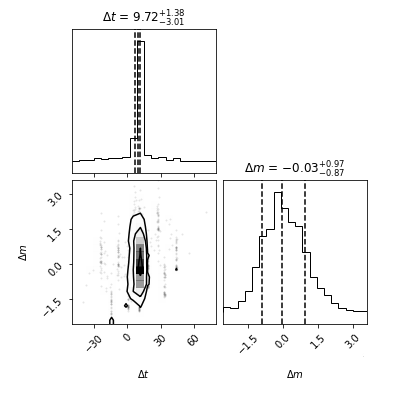
\includegraphics[width=0.6\linewidth]{microlensing/images/histo1.png}
	\caption{Гистограммы, построенные по 2500 значениям временных задержек $\Delta t$ и относительных усилений $\Delta m$.} 
	\label{fig:histograms}
\end{figure}

Гистограммы по всем значениям $\Delta m$ можно трактовать как распределение вероятности усиления (в звездных величинах) вследствие микролинзирования. Гистограммы по значениям $\Delta t$ иллюстрируют возможное влияние микролинзирования на точность оценок временных запаздываний между изображениями, и, как следствие, на точность определения постоянной Хаббла.

На картах, используемых в данной работе, источник чаще попадал в области без каустик, из-за чего для большого количества реализаций микролинзирование вообще никак не сказалось. Это объясняет высокий и узкий пик гистограммы около истинного значения $\Delta t$. Тем не менее, разброс по $\Delta m$ гораздо шире. Это означает, что в реальности затруднительно отделить макроусиление от линзы от микроусиления от отдельных звезд. Из этого можно сделать следующий вывод: в идеальных условиях, когда наблюдения производятся часто и при помощи идеального телескопа, вклад микролинзирования в значения временной задержки и относительного усиления по крайней мере между изображениями S1 и S2 SN Refsdal невелик. Также это может указывать на то, что ошибки величины $\Delta m$ в работах из обзора \cite{treu2016}, возможно, недооценены. %Ошибки в $\Delta t$ из-за микролинзирования сравнимы с ошибками самой величины. 

%Теперь увеличим количество различных положений сверхновой на карте: по 200 на каждой из них, всего 200х200=40000 реализаций. Но теперь только для плоского источника. Гистограмма по 40000 точек не очень сильно отличается от гистограммы для 2500 точек. Возможно, для полноценного статичестического исследования не нужно так много реализаций.


%Открытые вопросы: 
%(а) Будет ли вклад микролинзирования  плоского источника отличаться от гауссового? Для этого нужно знать, какой профиль яркости у SN Refsdal.
%(б) Будут ли ошибки такими же маленькими, если кривая блеска будет наблюдаться после пика или в другом фильтре? В идеале стоит проверить и то, и то, но хочется понимать, корректно ли работает данный алгоритм.
%(в) Есть основания полагать, что dt и dm должны быть скореллированы (например, как в (Kelly et al. 2016). Но нужно ли это учитывать при фиттировании?




